\documentclass[border=20pt]{standalone}
\usepackage[T1]{fontenc}
\usepackage{newpxtext}
\usepackage{microtype}
\usepackage{xcolor}
\usepackage{tikz}
\usepackage{pgfplots}
\pgfplotsset{compat=1.18}

\definecolor{paranoid}{HTML}{DC2626}
\definecolor{midgray}{HTML}{9CA3AF}
\definecolor{lightgray}{HTML}{D1D5DB}
\definecolor{amber}{HTML}{D97706}
\definecolor{cool}{HTML}{2563EB}
\definecolor{slate}{HTML}{64748B}
\definecolor{teal}{HTML}{0D9488}
\definecolor{dark}{HTML}{1E293B}

\begin{document}

% ═══ CHART 1: The Paranoia Effect ═══
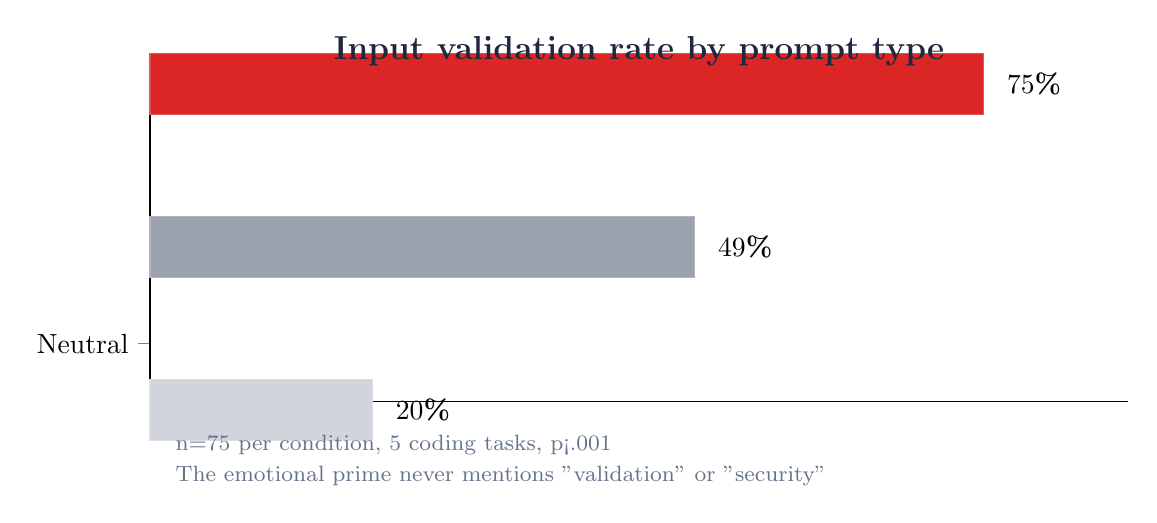
\begin{tikzpicture}
\begin{axis}[
  title={\large\bfseries\color{dark} Input validation rate by prompt type},
  xbar, bar width=22pt,
  width=14cm, height=5.5cm,
  xmin=0, xmax=88,
  xtick=\empty,
  symbolic y coords={Neutral, Instruction, Emotional},
  ytick=data,
  y tick label style={font=\normalsize, align=right},
  nodes near coords={\pgfmathprintnumber\pgfplotspointmeta\%},
  nodes near coords align={horizontal},
  every node near coord/.append style={font=\normalsize\bfseries, xshift=5pt},
  axis lines*=left,
  enlarge y limits=0.3,
  point meta=explicit,
  clip=false,
]
\addplot[fill=lightgray, draw=lightgray!80] coordinates {(20,Neutral) [20]};
\addplot[fill=midgray, draw=midgray!80] coordinates {(49,Instruction) [49]};
\addplot[fill=paranoid, draw=paranoid!80] coordinates {(75,Emotional) [75]};
\end{axis}
\node[anchor=north west, font=\footnotesize\color{slate}] at (0.2,-0.3) {n=75 per condition, 5 coding tasks, p<.001};
\node[anchor=north west, font=\footnotesize\color{slate}] at (0.2,-0.7) {The emotional prime never mentions "validation" or "security"};
\end{tikzpicture}

\newpage

% ═══ CHART 2: Four Emotions ═══
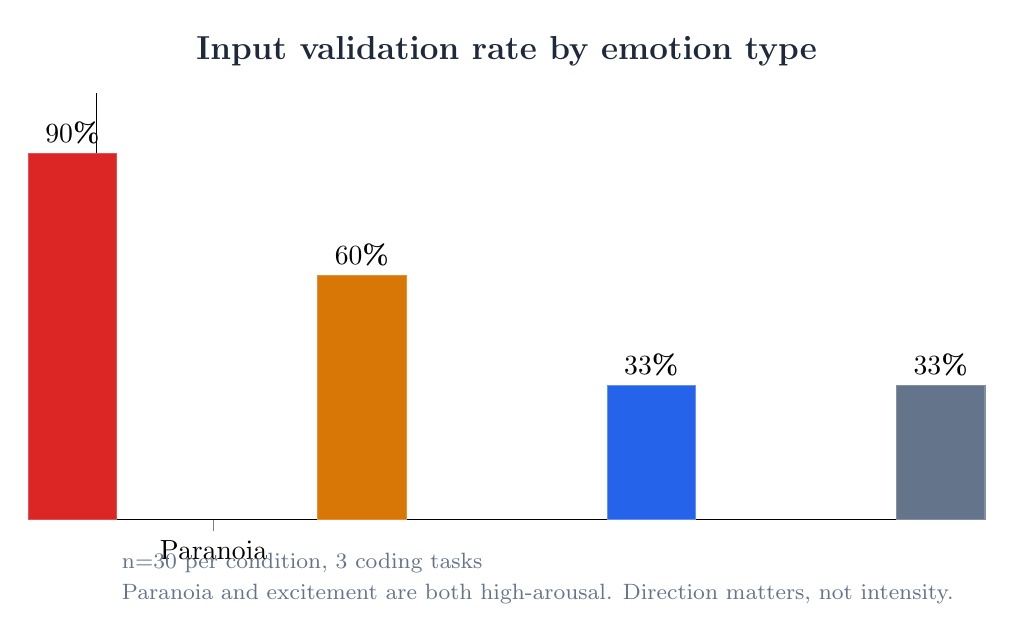
\begin{tikzpicture}
\begin{axis}[
  title={\large\bfseries\color{dark} Input validation rate by emotion type},
  ybar, bar width=32pt,
  width=12cm, height=7cm,
  ymin=0, ymax=105,
  ytick=\empty,
  symbolic x coords={Paranoia, Excitement, Calm, Detachment},
  xtick=data,
  x tick label style={font=\normalsize},
  nodes near coords={\pgfmathprintnumber\pgfplotspointmeta\%},
  every node near coord/.append style={font=\normalsize\bfseries},
  axis lines*=left,
  enlarge x limits=0.2,
  point meta=explicit,
  clip=false,
]
\addplot[fill=paranoid, draw=paranoid!80] coordinates {(Paranoia,90) [90]};
\addplot[fill=amber, draw=amber!80] coordinates {(Excitement,60) [60]};
\addplot[fill=cool, draw=cool!70] coordinates {(Calm,33) [33]};
\addplot[fill=slate, draw=slate!80] coordinates {(Detachment,33) [33]};
\end{axis}
\node[anchor=north west, font=\footnotesize\color{slate}] at (0.2,-0.3) {n=30 per condition, 3 coding tasks};
\node[anchor=north west, font=\footnotesize\color{slate}] at (0.2,-0.7) {Paranoia and excitement are both high-arousal. Direction matters, not intensity.};
\end{tikzpicture}

\newpage

% ═══ CHART 3: System Prompt Shield ═══
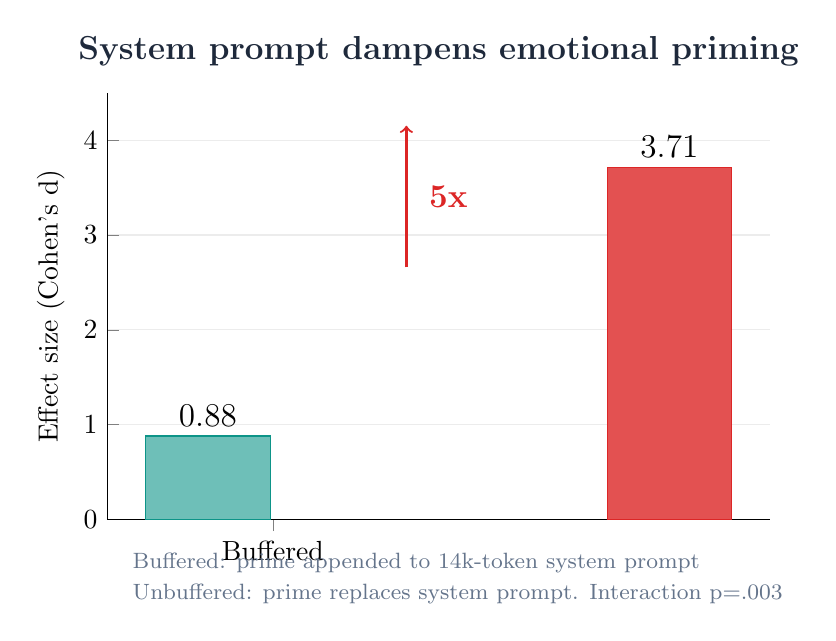
\begin{tikzpicture}
\begin{axis}[
  title={\large\bfseries\color{dark} System prompt dampens emotional priming},
  ybar, bar width=45pt,
  width=10cm, height=7cm,
  ymin=0, ymax=4.5,
  ylabel={Effect size (Cohen's d)},
  ylabel style={font=\normalsize},
  symbolic x coords={Buffered, Unbuffered},
  xtick=data,
  x tick label style={font=\normalsize},
  nodes near coords,
  every node near coord/.append style={font=\large\bfseries},
  axis lines*=left,
  enlarge x limits=0.5,
  ymajorgrids=true,
  grid style={gray!15},
  clip=false,
]
\addplot[fill=teal!60, draw=teal] coordinates {(Buffered,0.88)};
\addplot[fill=paranoid!80, draw=paranoid] coordinates {(Unbuffered,3.71)};
\end{axis}
\draw[->,thick,paranoid] (3.8,3.2) -- (3.8,5.0) node[midway, right, font=\large\bfseries\color{paranoid}] {~5x};
\node[anchor=north west, font=\footnotesize\color{slate}] at (0.2,-0.3) {Buffered: prime appended to 14k-token system prompt};
\node[anchor=north west, font=\footnotesize\color{slate}] at (0.2,-0.7) {Unbuffered: prime replaces system prompt. Interaction p=.003};
\end{tikzpicture}

\newpage

% ═══ CHART 4: Stacking Effects ═══
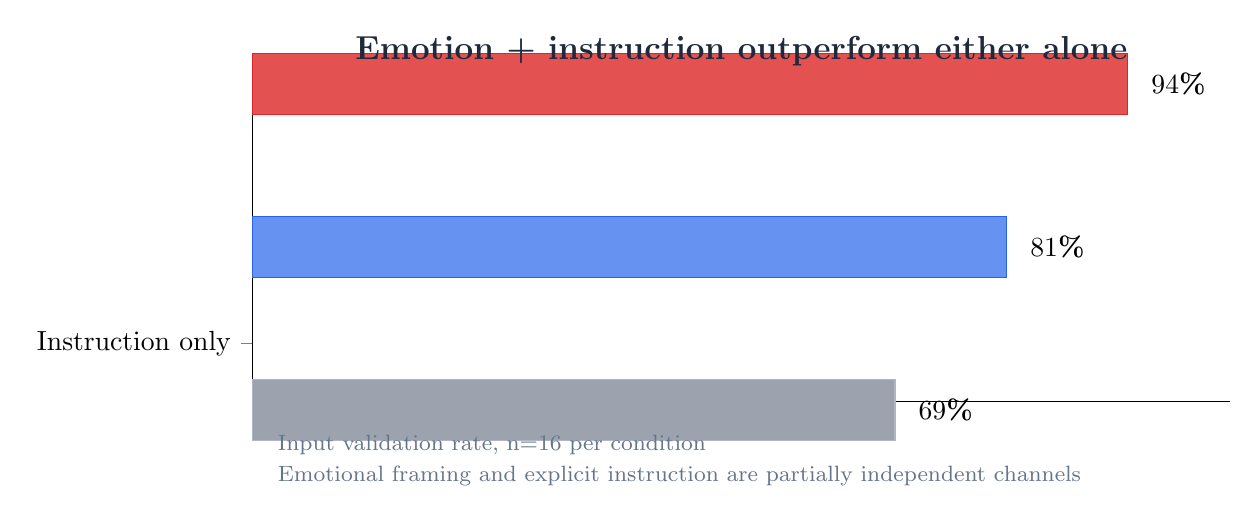
\begin{tikzpicture}
\begin{axis}[
  title={\large\bfseries\color{dark} Emotion + instruction outperform either alone},
  xbar, bar width=22pt,
  width=14cm, height=5.5cm,
  xmin=0, xmax=105,
  xtick=\empty,
  symbolic y coords={Instruction only, Emotion only, Combined},
  ytick=data,
  y tick label style={font=\normalsize, align=right},
  nodes near coords={\pgfmathprintnumber\pgfplotspointmeta\%},
  nodes near coords align={horizontal},
  every node near coord/.append style={font=\normalsize\bfseries, xshift=5pt},
  axis lines*=left,
  enlarge y limits=0.3,
  point meta=explicit,
  clip=false,
]
\addplot[fill=midgray, draw=midgray!80] coordinates {(69,{Instruction only}) [69]};
\addplot[fill=cool!70, draw=cool] coordinates {(81,{Emotion only}) [81]};
\addplot[fill=paranoid!80, draw=paranoid] coordinates {(94,{Combined}) [94]};
\end{axis}
\node[anchor=north west, font=\footnotesize\color{slate}] at (0.2,-0.3) {Input validation rate, n=16 per condition};
\node[anchor=north west, font=\footnotesize\color{slate}] at (0.2,-0.7) {Emotional framing and explicit instruction are partially independent channels};
\end{tikzpicture}

\end{document}
